\chapter{SleeveAR}
\label{sec:sleevear}

\section*{Summary}

Before implementing SleeveAR, it was vital to fully establish what were our goals and what we wanted to achieve. 
The following chapter describes our vision of this work and lists the feautures we considered to be a minimum requirement for a successful implementation.



\section{Vision}

\begin{figure*}[!t]
    \begin{center}
        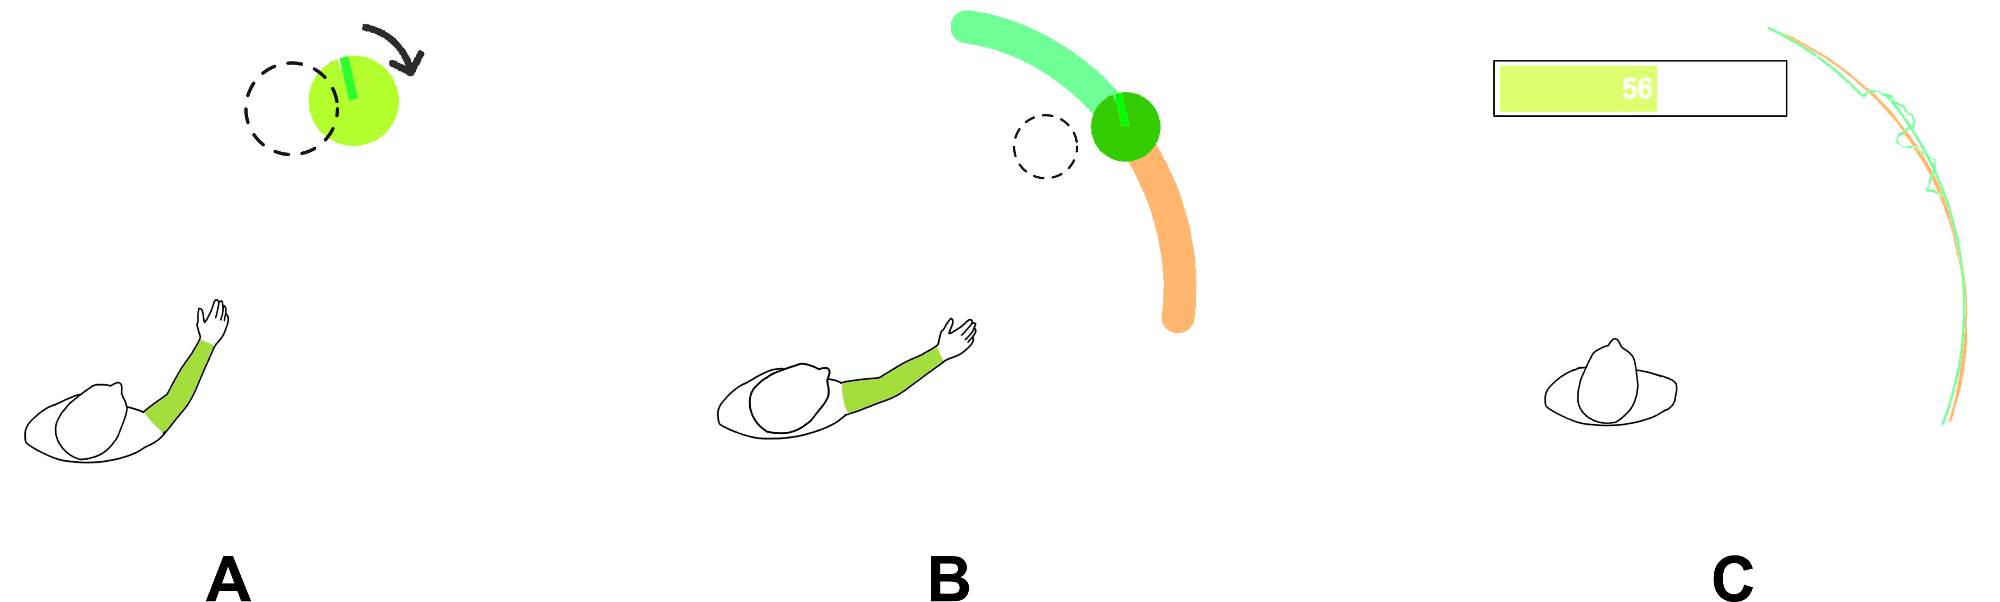
\includegraphics[width=0.9\textwidth]{imgs/interaction.png}
    \end{center}
    \caption{Sleeve Projected Feedback: A) bla. B) Bla. C) Bla}
    \label{fig:interaction}
\end{figure*}

SleeveAR aims further beyond the accomplishments LightGuide was able to make. 
As described in the previous section, Lightguide only focused on projecting information on top of the hand. Not only does this leave a small room for movement variety, but also the amount of possible information given can be quite reduced.
By increasing the projection area throughout the whole arm we can successfully improve an user's awareness while an movement is being executed. 
Not only that, but if it was possible for the movement being replicated to be originated by another person, we could achieve much more realistic and useful guidance.
With SleeveAR virtual content can be projected onto different surfaces, and even, onto people's own limbs, to provide, in real-time, a more immersive experience. 

Our vision consists on two main concepts. Firstly, the precise recording of the exercise being demonstrated by a personal therapist. 
And secondly, the ability to properly guide another person, the rehabilitation subject, during the execution of the pre-recorded exercise. 
While, at the same time, provide awareness of the rehabilitation exercise progress to insure the correctness of the patient's movements.
With SleeveAR, a therapist can easily demonstrate the prescribed exercises and make sure his patient will perform them correctly without the requirement of his close supervision.

In the SleeveAR system, the exercise being performed needs to be recorded beforehand, which, in this case, should be a health professional. 
Not only it provides a great range of possible movements, but also assigns,onto the professional, the responsibility of providing adequate exercises based on a specific patient's condition


\section{Visual Feedback}

Providing useful and minimalist design was our goal when designing our visual feedback. There were some key points we wanted to address when designing it.
First of all, the visual information had to provide the user with a representation of his \textbf{current} position, while also showing the \textbf{desired} position. 
These representations had to be done in a way the user would easily comprehend what to do in order to achieve that same desired position.
To provide suitable feedback regarding the full arm we first applied different design for each of the regions. Next we will present our planned visual feedback designs.

\subsection{Fore Arm}

\begin{figure}[!t]
    \begin{center}
        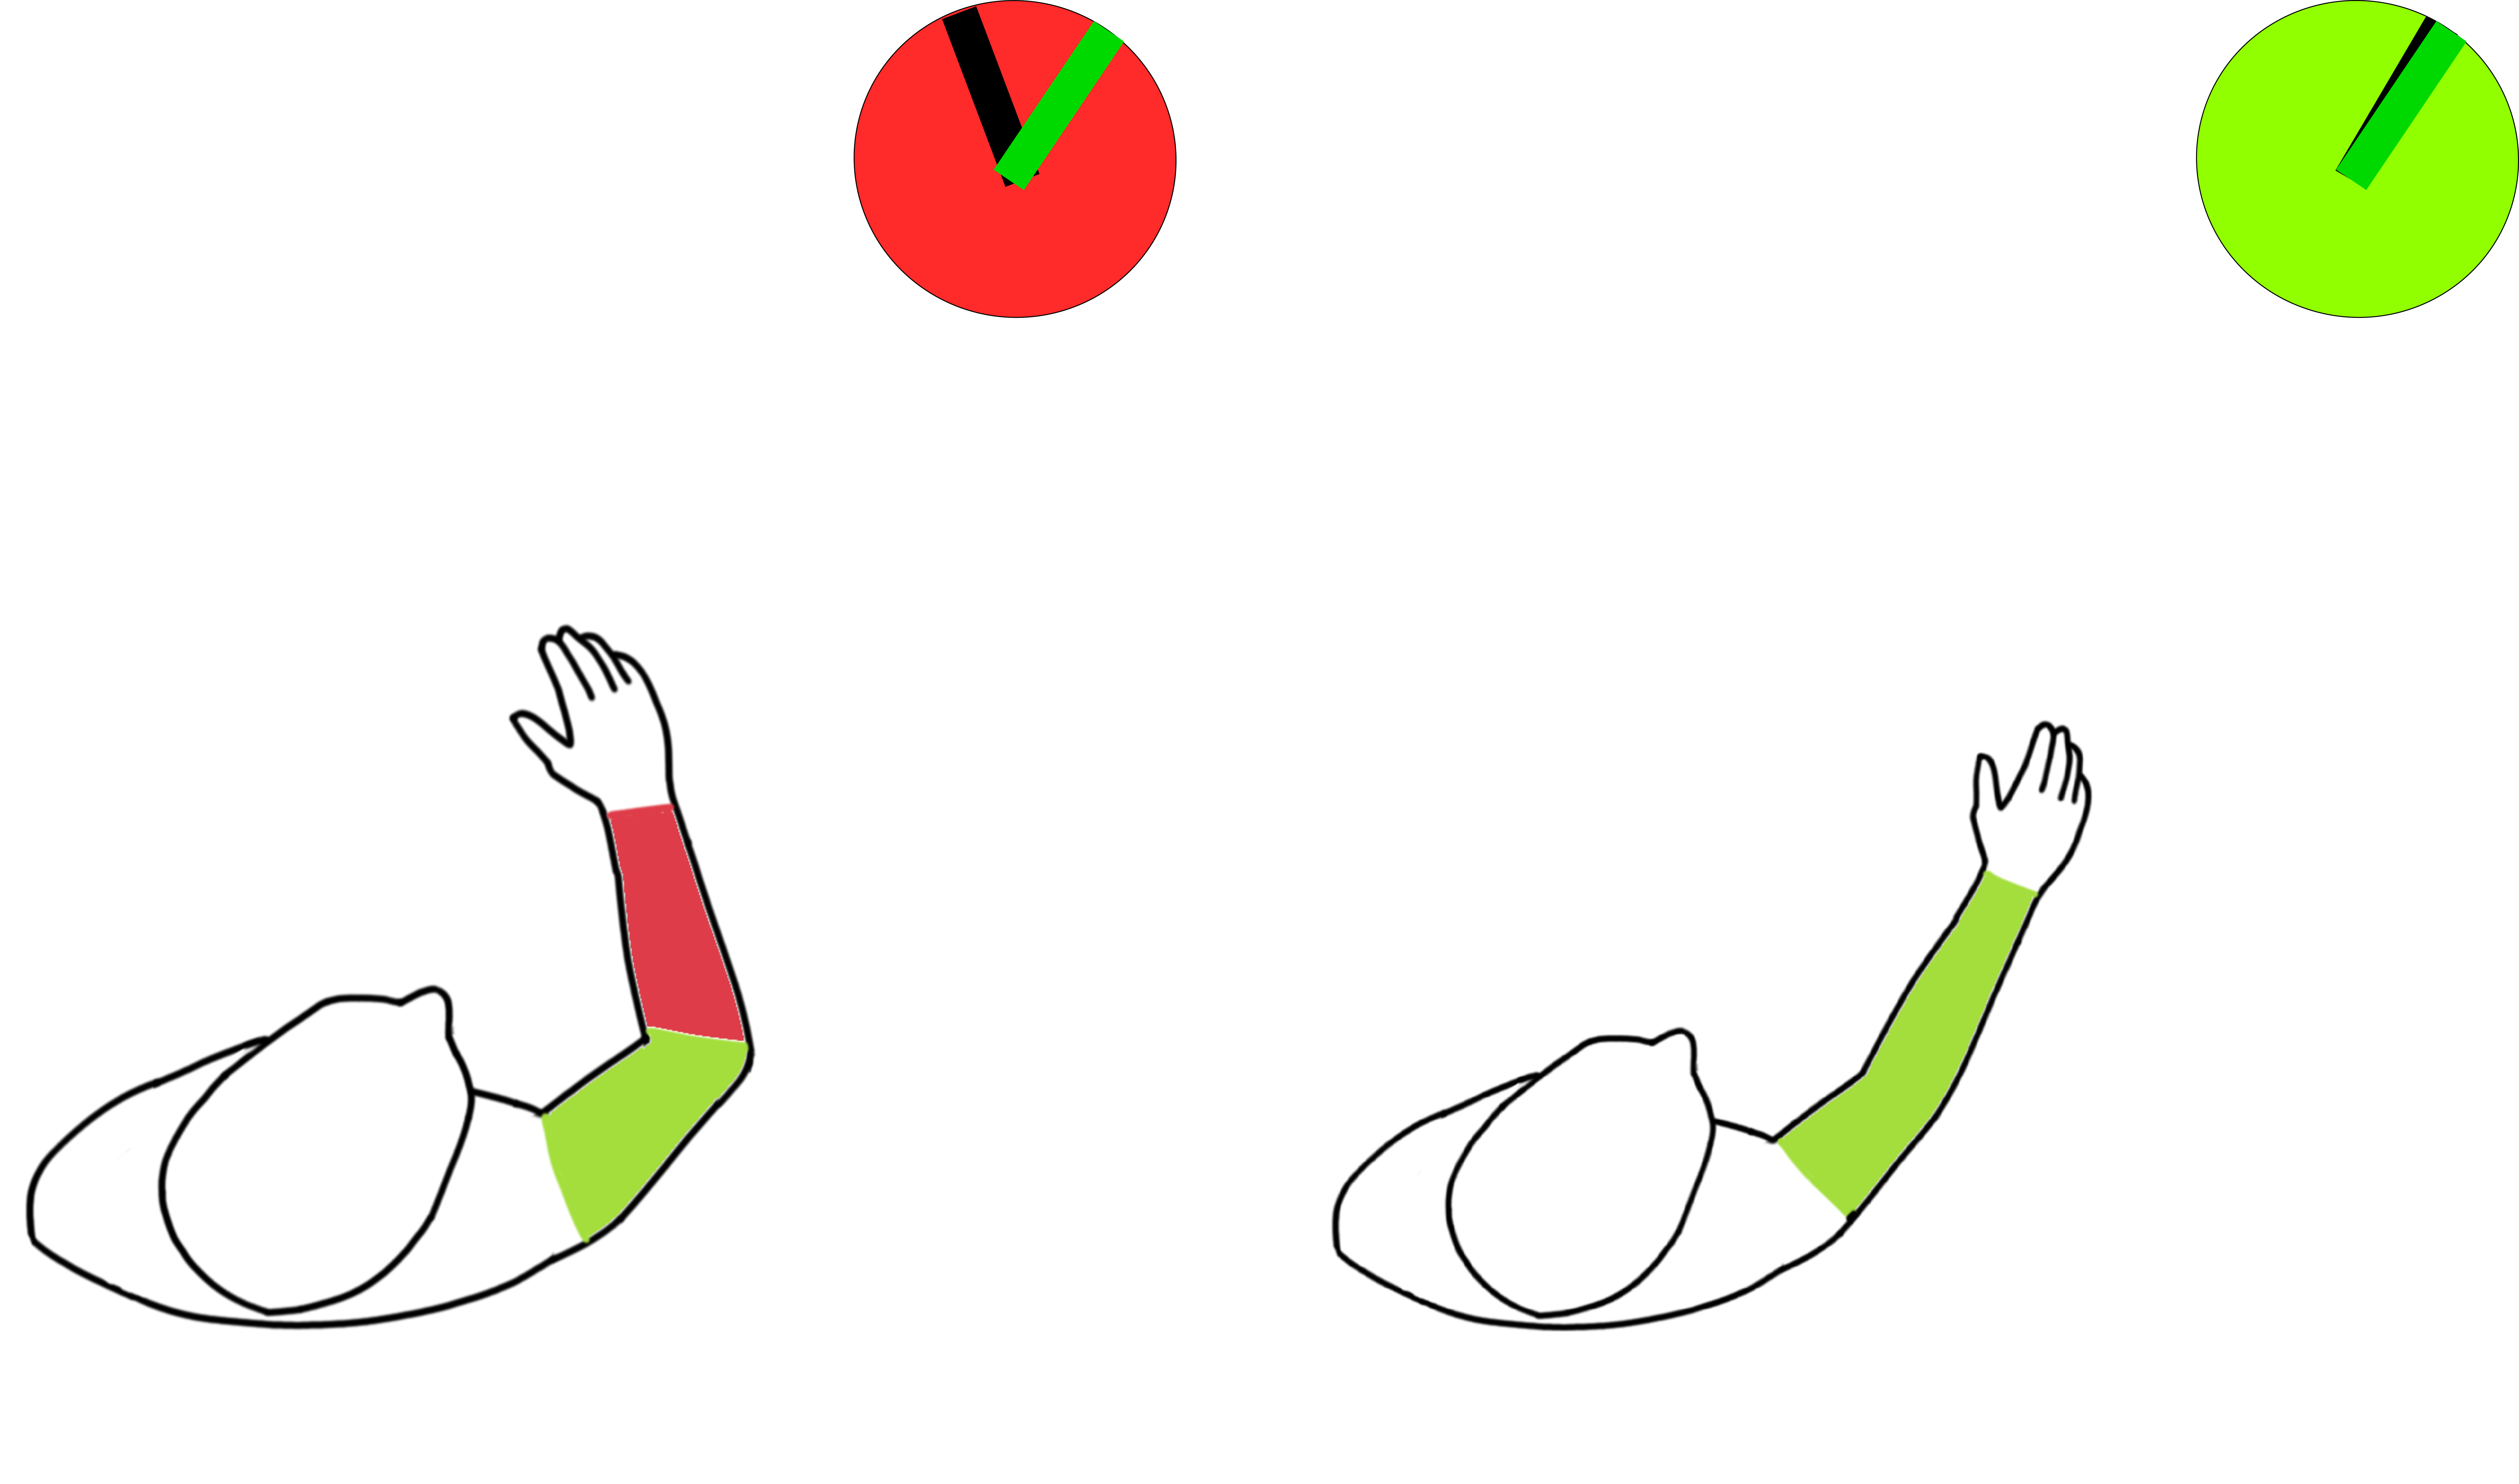
\includegraphics[width=0.5\textwidth]{imgs/forearmfeedback.png}
    \end{center}
    \caption{caption}
    \label{fig:forearmfeedback}
\end{figure}

Before creating the fore arm visual feedback it was important to understand what type of movement could be executed with this arm region.
The fore arm is connected to the upper arm by the elbow joint and its range of motion could be summarized in extension and flexing of the arm.
When extending or flexing the arm, we basically are changing the elbow angle, given by the angle between the upper and fore arm.
If we look at figure \todo{figura} we can see an example of a 90 degree arm flexing.

As we said previously, we wanted both designs to represent the current and desired state. Our final design for a fore arm feedback makes use of a circle with two bars, similar to a clock with two pointers.

%\subsubsection{Current State}

To represent the current state, we use the black bar, seen in figure \ref{fig:forearmfeedback}. Whenever the user moves his fore arm, this bar will move accordingly.

%\subsubsection{Desired State}

The desired fore arm state is represented by the green bar. For the user to achieve this state, is is required of him to move his fore arm in order for the black bar to reach the green bar.

%\subsubsection{Additional Information}

To extend the user's awareness we added two additional features specifically to this design. Depending on the distance between both bars, the circle color would fade between red, too far, and green, close enough. Also, if the black bar gets too far from the desired position, rotating arrows will appear to wan the user he is currently not correctly positioned. Next we present the planned design for the upper arm feedback.


\subsection{Upper Arm}

\begin{figure}[!b]
    \begin{center}
        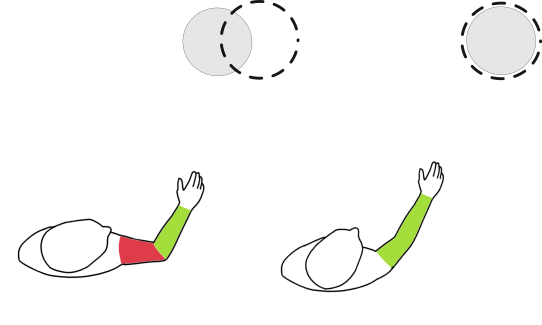
\includegraphics[width=0.5\textwidth]{imgs/upperarmfeedback.png}
    \end{center}
    \caption{caption}
    \label{fig:upperarmfeedback}
\end{figure}

As for the upper arm region, the type of movement allowed can be represented by the direction it is pointing to, which is obtained by a direction vector from the shoulder to the elbow as seen in fig \todo{figura}.
Once again, it was necessary for the design, seen at fig \ref{fig:upperarmfeedback} to both show the current and desired state. 

%\subsubsection{Current State}

To represent the upper arm current direction, a dotted circumference was chosen. By moving the upper arm vertically or horizontally, the dotted circumference should move, respectively, vertically and horizontally.

%\subsubsection{Desired State}

As for the desired state, a simple circle was chosen. For the upper arm to achieve the desired direction the user simply has to move it until the dotted circumference surrounds the circle.

\subsection{Full Arm}

Each one of the previouly presented designs are able to guide each arm region individually.
In order to guide a user to a full arm position, we combined both of them as seen on fig \todo{figura}

By replacing the grey circle, used on the upper arm's design, with the elbow angle circle from the fore arm's design, we are able to use both of them simultaneously. 

All these designs are able to guide the user to a specific, but static, position. For us to be able to guide a user throughout a movement, there need to be some changes on it.

\section{Movement Guidance}

\todo{refazer}
Hereafter, as depicted in Figure~\ref{fig:vision}, 
the patient follows all provided feedback to replicate the pre-recorded movement step-by-step, without ever seeing the exercise executed before.
The current position of the subject's arm is being constantly tracked in order to always provide real-time 
feedback based on how he should move it from that point.
Visual feedback is achieved by projecting light onto his full arm and surroundings. The projection on the arm will enable us to 
guide a subject through translations and rotations, using different kinds of visual cues to different situations. As for the projection on the subject's surrounding 
will serve the purpose of providing other useful information not directly connected to the movement itself. 
In Figure~\ref{fig:vision} we can observe a progress bar being projected on the floor. 
This bar not only provides the subject an understanding of how far in the exercise he is at the moment, but also helps the subject visualize the angle of movement he should be doing.
Audio and haptic feedback can help inform the subject about specific information, without making him loose his focus on the visual feedback.
The haptic feedback is used to quickly notify the subject of any vital information about the current state of the exercise. 
Awareness of erroneous movements is achieved mainly by the employment of vibration cues into the patient's arm.
Furthermore, for the purpose of timing, auditory feedback provide the subject with information regarding when to start or stop the exercise by using recognizable audio cues which represent those same actions.

Interactive phases(Figure~\ref{fig:interaction}):
\begin{itemize}
\item {\bf Initial Position Phase:}
\item {\bf Task Performance:}
\item {\bf Progress Report:}
\end{itemize}



\begin{figure}[!b]
    \begin{center}
        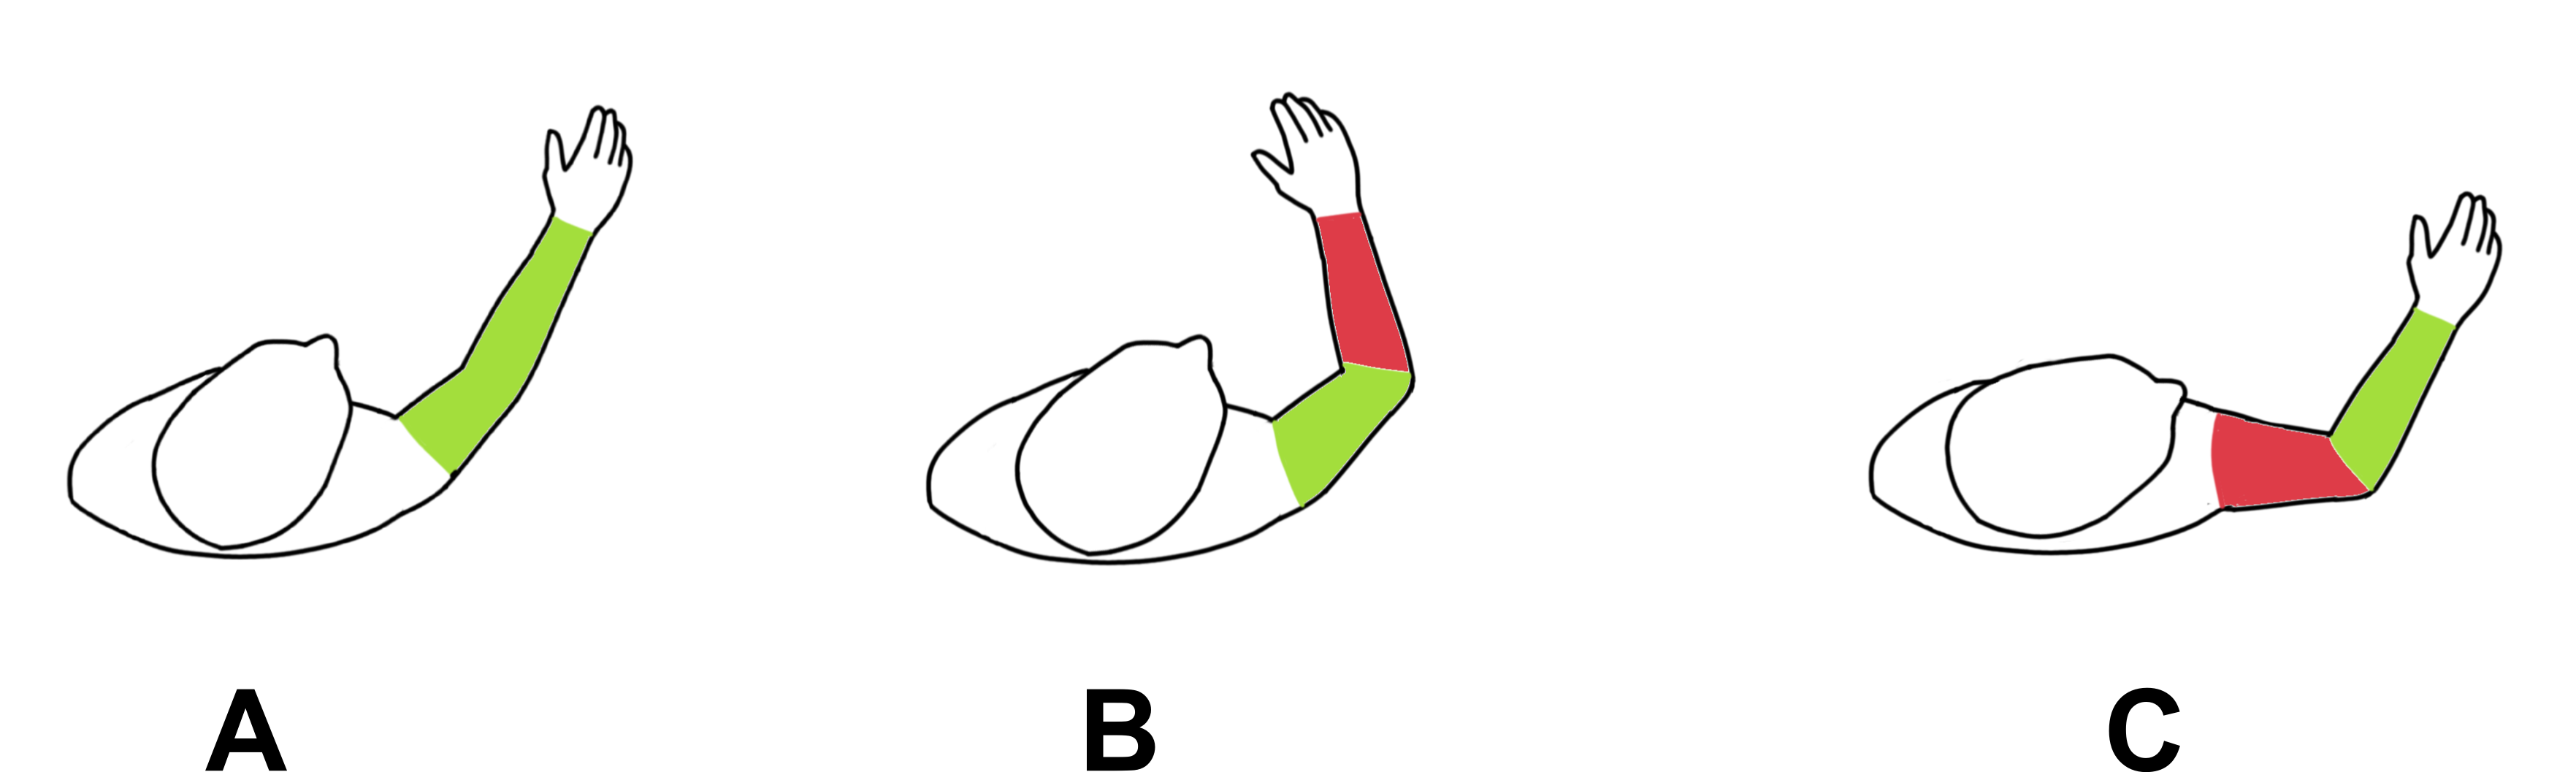
\includegraphics[width=\columnwidth]{imgs/visualfeedback.png}
    \end{center}
    \caption{Sleeve Projected Feedback: A) bla. B) Bla. C) Bla}
    \label{fig:vision}
\end{figure}